\chapter{Details of the IBM study}
\label{app:IBM}

In the case of the \emph{IBM} study, our published paper \cite{Aranda2007b} did not include all of our findings due to space constraints. The study is summarized in section \ref{sec:IBM}; this appendix expands on its motivation and findings.


\section{Motivation}

Large-scale software development is characterized by the involvement of an inordinate number of people with very different backgrounds, skills, goals, and needs. The members of the software team are united by a set of common goals---such as the delivery of the software application---and reaching these goals demands from them the creation and communication of detailed project information to their colleagues. The nature of this project information is vast and heterogeneous, and may be as overarching as requirements specifications, or as seemingly trivial as the phone number of a colleague or the location of a library file in a repository.

For these projects, no team member needs to know every piece of information. Indeed, one could claim that it is impossible for any one member to know everything about their project. However, each of them depends on knowledge generated by people other than themselves, and their aggregated information-seeking and information-sharing activities form a web of interaction with one main purpose: improving the team's shared understanding of their project.

Reaching this shared understanding is considerably difficult, even for small teams. One of the main reasons for this difficulty is that communication of information seems deceptively simple. We often assume that the act of sending information, or that of making information available to other parties, is enough to ensure communication. Yet even the simplest models of communication available require a receiver to decode and assimilate the message for the communication instance to be considered successful. A communication event does not end with the transmission of a message; speaking (or writing) is not the same as communicating.

Reaching shared understanding, then, involves the effective use of social, organizational, and cognitive elements, even for fields as seemingly technical as software development. Shared understanding cannot be developed systematically: the production of documents, such as requirements specifications, is meaningless if their content is not decoded and internalized by their readers. Furthermore, shared understanding can never be guaranteed: we cannot ensure that two parties have a shared understanding; we can only point to interactions in which the lack of understanding became apparent through breakdowns and conflicts.

If the development of shared understanding is difficult for small teams, the task becomes monumental for large-scale software development. In these settings, software teams are geographically separated, their members number in the hundreds or thousands, their skills and vocabularies are extremely specialized and widely divergent, and they must battle with many forces that continuously or suddenly attempt to shift the course of the project.

But the difficulty of the task does not make it any less vital. Without reaching enough shared understanding, a software team will not be working consistently towards the same goals; it will be surprised by obstacles that should have been visible to their members; and it will cause economic losses for the company, and low quality products for its customers. On the other hand, the development of shared understanding will focalize the efforts of the full team, improve the flow of information within and from outside its boundaries, and improve the organization's opportunities in the market. Reaching shared understanding, then, is a necessary, if not a sufficient, requirement for the success of a software development team.

In this study we explored a strategy to analyze shared understanding dynamics in large teams that draws from cognitive and organizational theories, as well as Kruchten's 4+1 views of software architecture. We argue for the analysis of large software teams using several views: structural, process-based, dependency-based, social, competency-based, artifact-based, intentional, physical, and scenario-based. 

The study of shared understanding in a software team raises, first, a problem of completeness: it is realistically impossible to record and analyze all of the relevant data and all the interactions of teams of even modest sizes. As researchers, we need to focus our attention in a limited subset of all possible data, and to minimize the impact of this data incompleteness issue.

Several researchers have addressed this problem by analyzing small but significant interactions among people, or between people and machines. These analyses have produced valuable insights into the nature and efficacy of some specific phenomena of group and human-computer interaction, such as ship navigation \cite{Hutchins1995} or communication between remote sites. However, they do not provide a broad picture of effective shared understanding dynamics, nor explain how these specific phenomena affect and are affected by other events that are commonplace in group interactions.

A second problem of the study of shared understanding is the difficulty of observing its development. As mentioned earlier, it is impossible, at least given our current technology, to confirm that two people share the same understanding of a situation---as long as no conflict or breakdown appears between them, their understanding will seem to be functionally equivalent. It is only in moments of breakdown that a lack of understanding becomes evident.

The researcher of shared understanding, then, needs to focus on those activities and interactions that open a possibility to study the changes in understanding in one or more involved parties: learning instances, communication of previously unknown information, misunderstandings, breakdowns, recoveries, and others. Given the informal and unexpected nature of many of these events, field studies are essential components of our research.

Finally, a third challenge of studying shared understanding is that team members have a wide variety of alternative mechanisms to facilitate it, and they all must be included as part of the study to get an accurate impression of the effectiveness of each dynamic. An exclusive focus, for example, on processes and methodologies will ignore the informal interactions (such as water cooler conversations) that play a large role in strengthening the understanding in a team; a focus on the latter will equally suffer from ignoring the processes that, unknown to the researcher, every team member has internalized as part of their understanding. Similarly, an emphasis on documents ignores the effect of face to face communications, and vice-versa.

As a response to these challenges (incompleteness of information, lack of observability, and breadth of shared understanding strategies), we developed a multiple-view approach to study the development of shared understanding in large software teams. Details of our proposal are summarized in the following section.

\section{Organizational Views}

The problem of studying the development of shared understanding in large software teams depends on a more fundamental problem: how to reason systematically and holistically about software development dynamics?

The study of these dynamics (software methodologies, best practices, project management techniques, etc.) is currently characterized by the narrow view with which it approaches the phenomenon under investigation. Business processes, for instance, are often engineered with little regard for the people that will execute them, their skills, or their geographic locations. Software development practices, such as code reviews or pair programming, are usually studied in isolation from a number of factors that severely affect or are affected by their adoption in a development team.

In some cases, this narrow view is beneficial. It allows researchers to pull apart one phenomenon from the complex mess that is software development, and to study it in detail. But in other cases a simplistic view is not only naive, but counterproductive, leading the researcher to short-sightedly collect incomplete data and reach false conclusions.

The study of shared understanding falls in the latter category, since it depends as much on team processes as on social networks; on documents and models as on the skills and terminology of the people reading them; on project requirements as on the tacit knowledge that lets developers estimate and prioritize them satisfactorily.

However, our community does not currently have a framework to make sense of these disparate elements of software development dynamics. Although we have concepts, languages, and diagrams to discuss several of these elements independently, we do not have the habit, or the means, to reason about them systematically and holistically.

Therefore, in order to study the development of shared understanding, we need to work simultaneously towards a framework that incorporates several views that are essential to this phenomenon. As this framework evolves, our knowledge of shared understanding will feed from this evolution and will, in turn, affect the development of the framework.

This is not the first time that studies in a software engineering field have needed to combine multiple aspects of analysis. The success of a similar approach in software architecture should be of use for the study of shared understanding. We refer to Kruchten's ``4+1 view model'' of software architecture \cite{Kruchten1995}. Kruchten identifies the problem caused by the ambiguity and narrowness of several approaches to model software architectures: ``sometimes the architecture of the software suffers scars (...) from an over-emphasis on one aspect of software development: data engineering, or run-time efficiency, or development strategy and team organization.'' In response, Kruchten proposes ``to organize the description of software architecture using several concurrent views, each one addressing one specific set of concerns.''

The complexity of the phenomenon of shared understanding, and the qualities of Kruchten's model, suggest that an approach similar to his own should be fruitful for our domain. A diversity of views is needed when analyzing something as complex as large-scale software development. These views need to cover the technical, social, cognitive, and organizational factors that impact software development, and their combined application should convey a holistic picture of the software development team under study.

As part of our studies of shared understanding, we prepared a preliminary version of this multiple-views model of organizations. The organizational views that we propose are the following:

\textbf{Structural view.} The first view we propose is one that displays the structural hierarchy of the software development organization. This management structure may seem trivial, and it is for small teams, but large groups have complex hierarchical and team structures that affect the development of software deeply. Each individual's development and per-formance goals are often assigned from higher hierarchical levels, and when every individual needs to satisfy an n-dimensional matrix management structure, we need to study and understand this hierarchical context if we want to propose sensible refinements to the organization.

Information about the management structure of an organization is relatively easy to obtain. To some extent, it serves as a framework to relate the other views and roles to specific elements in the organization. However, note that we cannot represent the structural view with a simple hierarchy tree, as it fails to represent matrix structures easily.

\textbf{Process view.} As its name suggests, the process view focuses on the relevant business processes that are executed as part of the operation of the company. It is, perhaps, the most commonly used perspective to describe an organization in the IT industry, and it is also the one that has been better developed. Languages such as BPML can be used extensively to communicate this type of information, and frameworks such as RUP prescribe how to manage it.

Modeling an organization's processes brings up an important question: should the analyst focus on the processes as specified (that is, as they are supposed to happen), or on the processes as executed (as they truly happen)? On one hand, although the two often overlap, the real-world execution of processes tends to skip irrelevant steps, to take shortcuts if needed, or to be aided by tacit or intangible activities that cannot be modeled easily. On the other hand, analyzing processes as specified is more straightforward, as it is likely that, at least in large organizations, these processes have already been agreed upon and documented by key stakeholders.

For this view, we propose to focus on processes as executed instead of as specified, if at all possible. Although this increases the troubles for the analysis of business processes, it also increases the validity and power of its findings.

\textbf{Dependency view.} Software products in large companies have an inordinate amount of dependencies to other projects. Their successful completion depends on the completion of products built by other teams, located in or outside the same organization, which in turn depend on a number of other products built by yet other parties. The chain of dependencies becomes quickly complicated---the number of third-party dependencies for large products may well number in the thousands, and their impact on the success or failure of these products is highly significant. Similarly, the number of products that depend on the project under analysis may be considerable as well, and it is reasonable to expect that these dependent parties have a vested interest in being informed about the progress of their dependees and in influencing their activities.

Although some companies have successfully found ways to document and keep track of the dependencies of their projects through dependency management applications, the view of a software product as an entity that is mostly detached from other projects is still prevalent in academic discussions of software development. Satisfying the time and requirements constraints requested by a product's dependent projects demands a considerable effort. Hence, studying the development of shared understanding for these companies requires the analysis of product dependencies, of the mechanisms through which they are discovered and negotiated, and of the ways in which they are managed as part of product development.

\textbf{Social view.} The social view focuses on the formal and informal interactions between stakeholders of a software project, and on the social structures in which they are arranged.

Through the use of Social Network Analysis, we can analyze the structural and dynamic qualities of software teams, and explore the ways in which interactions take place in practice (as opposed to the ways in which they are prescribed by business processes). Group characteristics, such as centrality and density, provide helpful metrics of group qualities. Techniques such as blockmodelling allow for the clustering of nodes based on their similarities in several networks. Concepts inspired by Social Network Analysis, such as knowledge transfer and social capital, provide additional insights to the study of interactions of software teams.

The study of social networks is of particular relevance to large-scale software development teams because many of their members serve the primary goal of facilitating the flow of information among social clusters. These individuals bridge the gaps between groups with different vocabularies, skillsets, and expectations. As a research community, we know very little of how these bridges carry out their tasks and ensure that product development runs smoothly.

\textbf{Competencies view.} The competencies view provides an inventory of the skills, background knowledge, and experience of the members of the software team. It is relevant because large teams develop highly specialized roles and competencies, and these usually imply distinct terminologies and subcultures. An awareness of these personal differences will be of importance when restructuring teams, providing opportunities for learning, and analyzing the feasibility of the implementation of best practices and team dynamics.

\textbf{Artifact view.} The artifact view allows us to investigate the qualities, affordances, and capabilities of the artifacts used in everyday software development. These artifacts (documents such as requirements specifications, or tools such as IDEs) are often focal points of communication and cognition, and hence their characteristics have a significant impact in software development activities.

The thorough study of all documents and tools used in a software project is not practical. But collecting data on the frequency with which different types of documents are used and their relevance for each group member may provide us with useful patterns of interaction and team dynamics. It will also point to particularly relevant documents, which may be studied with a more careful detail.

\textbf{Intentional view.} Tied to the social actors and to their positions in the organization's structure, the intentional view makes explicit the key goals (and means to achieve them) of a socio-technical system's agents. This perspective allows us to address questions such as: what are the goals of each agent? Are they currently satisfied or denied? What are the consequences of the interactions of the actors? And, perhaps more importantly, which structural arrangement suits best the satisfaction of as many goals as possible?

The study of the intentionality of social agents has advanced considerably. Some current proposals, such as the i* framework \cite{Yu1997}, provide analysts with the tools to apply the intentional view to socio-technical contexts. At the same time, large-scale uses of these proposals have so far resulted in cumbersome intentionality models that do not facilitate analysis. Considering the overwhelming number of agents and goals that are involved in large-scale software development, refinements to these intentionality proposals appear necessary if they are to be used for the study of shared understanding in these contexts.

\textbf{Physical view.} The physical perspective allows us to consider the actual physical and geographical context in which software development activities take place. It is perhaps the most overlooked perspective in software development studies, possibly because we tend to believe that electronic communications solve the problems caused by distance and location.

However, the challenges to software development that arise because of essentially physical circumstances are considerable: reduction of communication capabilities due to time zone differences, loss of richness of communication when switching from co-located to remote environments, and a lack of team culture caused by isolation are but three examples of problems inherent to physical distance and layout. There are indications that these issues are determinant factors of success or failure of software development projects. For these reasons, the physical view should be included in any holistic approach to the study of software development.

\textbf{Scenario-based view.} The eight views proposed so far are valuable by themselves, but they are likely to interact in ways that our separate perspectives cannot convey. Therefore, we propose an additional view, the equivalent of Kruchten's ``+1'' proposal: a scenario-based view that ties the rest together and provides a unified perspective of phenomena related to software development.

The scenario-based view explains how an event is handled from its initial trigger to its final consequences. It represents, in a way, ``executing'' the socio-technical system, and tracing it along all the other views of our proposal.

By necessity, the scenario-based view will be incomplete. It is impractical, and perhaps impossible, to capture the details of the execution of every event through the organization. We should be concerned with the normal and extraordinary execution of a few key scenarios that illustrate an aspect of the business' operation, not with the totality of scenarios and their consequences. But this incompleteness should not be interpreted as a deficiency that is exclusive of our proposal: any other approach to the study of large-scale software development will be either unworkable or incomplete as well (by ignoring either some of the views we propose or some of the instances in which they are used).


\section{Design and execution}
\label{sec:IBMDesign}

We conducted a study on shared understanding during the second half of 2006, with the dual purpose of learning insights on this concept and of assessing the validity of our approach. The subject of our pilot study was the project management team of a large software division. Our study focused on the social and structural views of the team's operation---the other views were incorporated to our proposal as their need was made apparent by our findings.

The project management team that was the subject of our studies is a group with high impact and high volume of interaction within the division. It oversees product development and serves as a bridge between ``technical'' and ``business'' people. This bridge role requires from them, in addition to advanced project management skills, a familiarity with at least two different professional cultures, vocabularies, and goals. They are focal enablers of shared understanding in the division, in the sense that they are the main point of contact for developers to learn product requirements, and for managers to learn their projects' status.

For these reasons, the people at the project management team have experienced the need to create roles, team dynamics, and processes that help them handle their responsibilities and coordinate the efforts of the full division towards shipping their releases.

We designed our study to explore these phenomena. We interviewed nine members of the project management team with a structured questionnaire that probed the applicability of some social network analysis, artifact analysis, and conceptual sketching techniques to the study of large-scale software development. The design of our pilot study allowed us to evaluate both the nature of shared understanding in this project management team, and the viability of our empirical techniques. Regarding the latter objective, the partial success of some of these techniques (for instance, our conceptual sketching questions proved to be too vague as stated, and while some of our Social Network Analysis questions were fruitful, some caused confusion) provided us with the insights necessary to, first, refine our techniques, and second, incorporate views that were not considered under the initial scope of our study.


\section{Results and observations}

The data from our study led to several observations on the nature of shared understanding dynamics in this project management team, which are summarized in the following paragraphs.

\textbf{Unidirectionality of team communications.} Although we expected the project management team to perform a bi-directional communication role between business and technical groups, and although this is consistent with the de facto perception of the team, our social network data points in a different direction. Figures \ref{fig:Consumers} and \ref{fig:Producers} represent the networks of information consumers and information producers related to the project management team. Red (darker) circles indicate people and groups outside the project management team.

\begin{figure}[tbp]
\centering
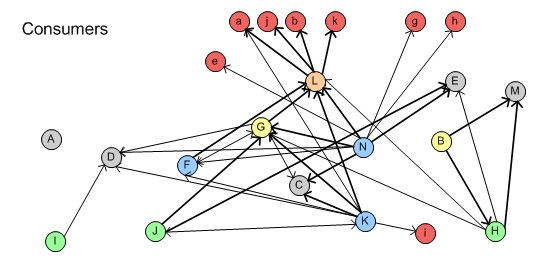
\includegraphics[scale=0.8]{consumers}
\caption{\label{fig:Consumers}IBM Study: Information consumers network}
\end{figure}

\begin{figure}[tbp]
\centering
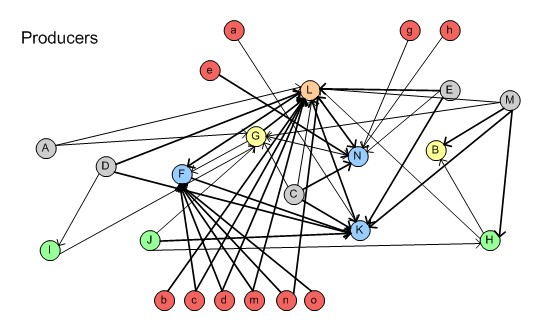
\includegraphics[scale=1.0]{producers}
\caption{\label{fig:Producers}IBM Study: Information producers network}
\end{figure}

Figure \ref{fig:Consumers} corresponds to the consumers' network. It represents, according to each node in the graph, who consumes the information produced by that person. Figure \ref{fig:Producers} corresponds to the producers' network. It represents (again, according to each node/person) who produces the information consumed by each person in the team. If all perceptions were equal, and if we had information from all relevant stakeholders, the second network should be equivalent to the first.

Figure \ref{fig:Mixed} mixes the first two networks, to obtain an information exchange network. It should be noted that the red (darker) nodes in the bottom, which correspond to technical groups and people, produce information that the project management team consumes, and this team then produces information that the red nodes in the top (business groups and people) consume. This was an unexpected pattern - as stated above, information flow in this team was supposed to be bidirectional between business and technical groups, not to flow mostly from technical to business people.


\begin{figure}[tbp]
\centering
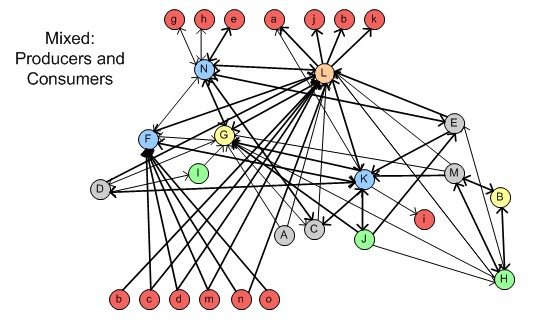
\includegraphics[scale=1.0]{mixed}
\caption{\label{fig:Mixed}IBM Study: Merged consumers and producers network}
\end{figure}

When we analyzed this pattern in greater detail, we found that people in the project management team do in fact communicate information from the business to the technical teams, but mostly at the start of a release cycle. The frequency and relevance of these communications are low. We believe this pattern might be a symptom of a disconnect between user needs and developer perceptions, which merits a closer analysis. This symptom is compounded by the following finding.

\textbf{Abstracted definition of success.} Almost all members of the project management team described their success criteria as shipping releases on time, with the expected features and the expected level of quality. However, nobody described success in terms of user satisfaction, or of meeting client expectations. The functional definition of success used by the team abstracts those considerations away.

This is problematic, since user needs and user requests go through close to a dozen ``hops'' until they reach the developers in charge of implementing them. If relevant information about satisfaction criteria or the intentions behind a requirement is dropped along the way, developers have no means to determine what it is that clients truly want.

We expected to find the project management team performing a ``client representative'' role in its interactions with the developers, but our data do not support this pattern. The ``client representative'' role may be performed by other teams in the division, but our data do not indicate whether these other teams do in fact communicate user concerns to developers, or if they rely on the release team to do so.

\textbf{Role specialization.} A few years ago, this project management team started to define its roles in greater detail, and to specialize its members. Today, the team seems to have a strong sense of the types of activities and responsibilities of each role. We have two types of evidence supporting this finding.

First, we asked every participant to sketch the structure of their team. In almost every case (except for the most recent additions to the team), the internal team structure was consistently well understood, even though few participants seem to have a strong picture of the relationship between the release team and the rest of the software division.

Second, the collaboration network of the team (shown in figure \ref{fig:Collaborators}) suggests a few very close collaborations as expected by those participants' roles, and a few weaker collaborations to other team members. Furthermore, comparing this network to the information exchange network (displayed above) shows that, although members collaborate with only a few people, they depend on many more to produce information essential for their activities. We believe this is an indication of a mature collaboration system in place.

\begin{figure}[tbp]
\centering
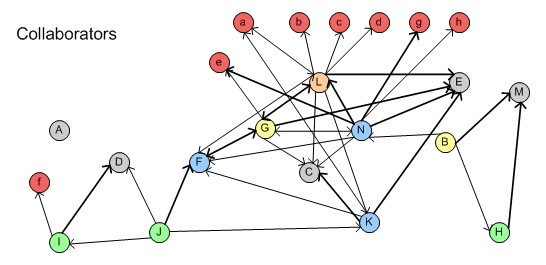
\includegraphics[scale=1.0]{collaborators}
\caption{\label{fig:Collaborators}IBM Study: Collaborators network}
\end{figure}

\textbf{Under-recognized role of interns.} Interns seem to do important (though perhaps routine) tasks, and to obtain as good a perception of the team dynamics as the managers in the team if they spend enough time working in it. Recruitment of interns for permanent positions might speed up considerably the learning curve involved in understanding the interactions and operations of a human system as complex as a software division. However, interns are rarely mentioned by other team members, and their mentorship is very informal. Based on our findings, we believe that a closer attention to the role and relevance of interns will be beneficial to the long-term efficiency of the project management team.

The findings reported above are, necessarily, an incomplete picture, since we restricted our analysis to a small team within a very large software division. A large scale study of the full division should yield insights with a much greater impact for its operation.

The study demonstrated the benefits of paying attention to the social and structural aspects of large-scale software development, but it also displayed the limitations of maintaining a narrow view of these phenomena. Although social and structural elements are major factors of software development and are worthy of consideration, the partial view they provided us with needed to be complemented with information about processes, physical location of team members, and the other perspectives described above. The proposal delineated in this appendix is the result of incorporating those ``missing perspectives'' into the study of shared understanding of software teams.

